\blankpage

\thispagestyle{empty}
\clearpage
\begin{tikzpicture}[remember picture, overlay]
\node at (3,-7) {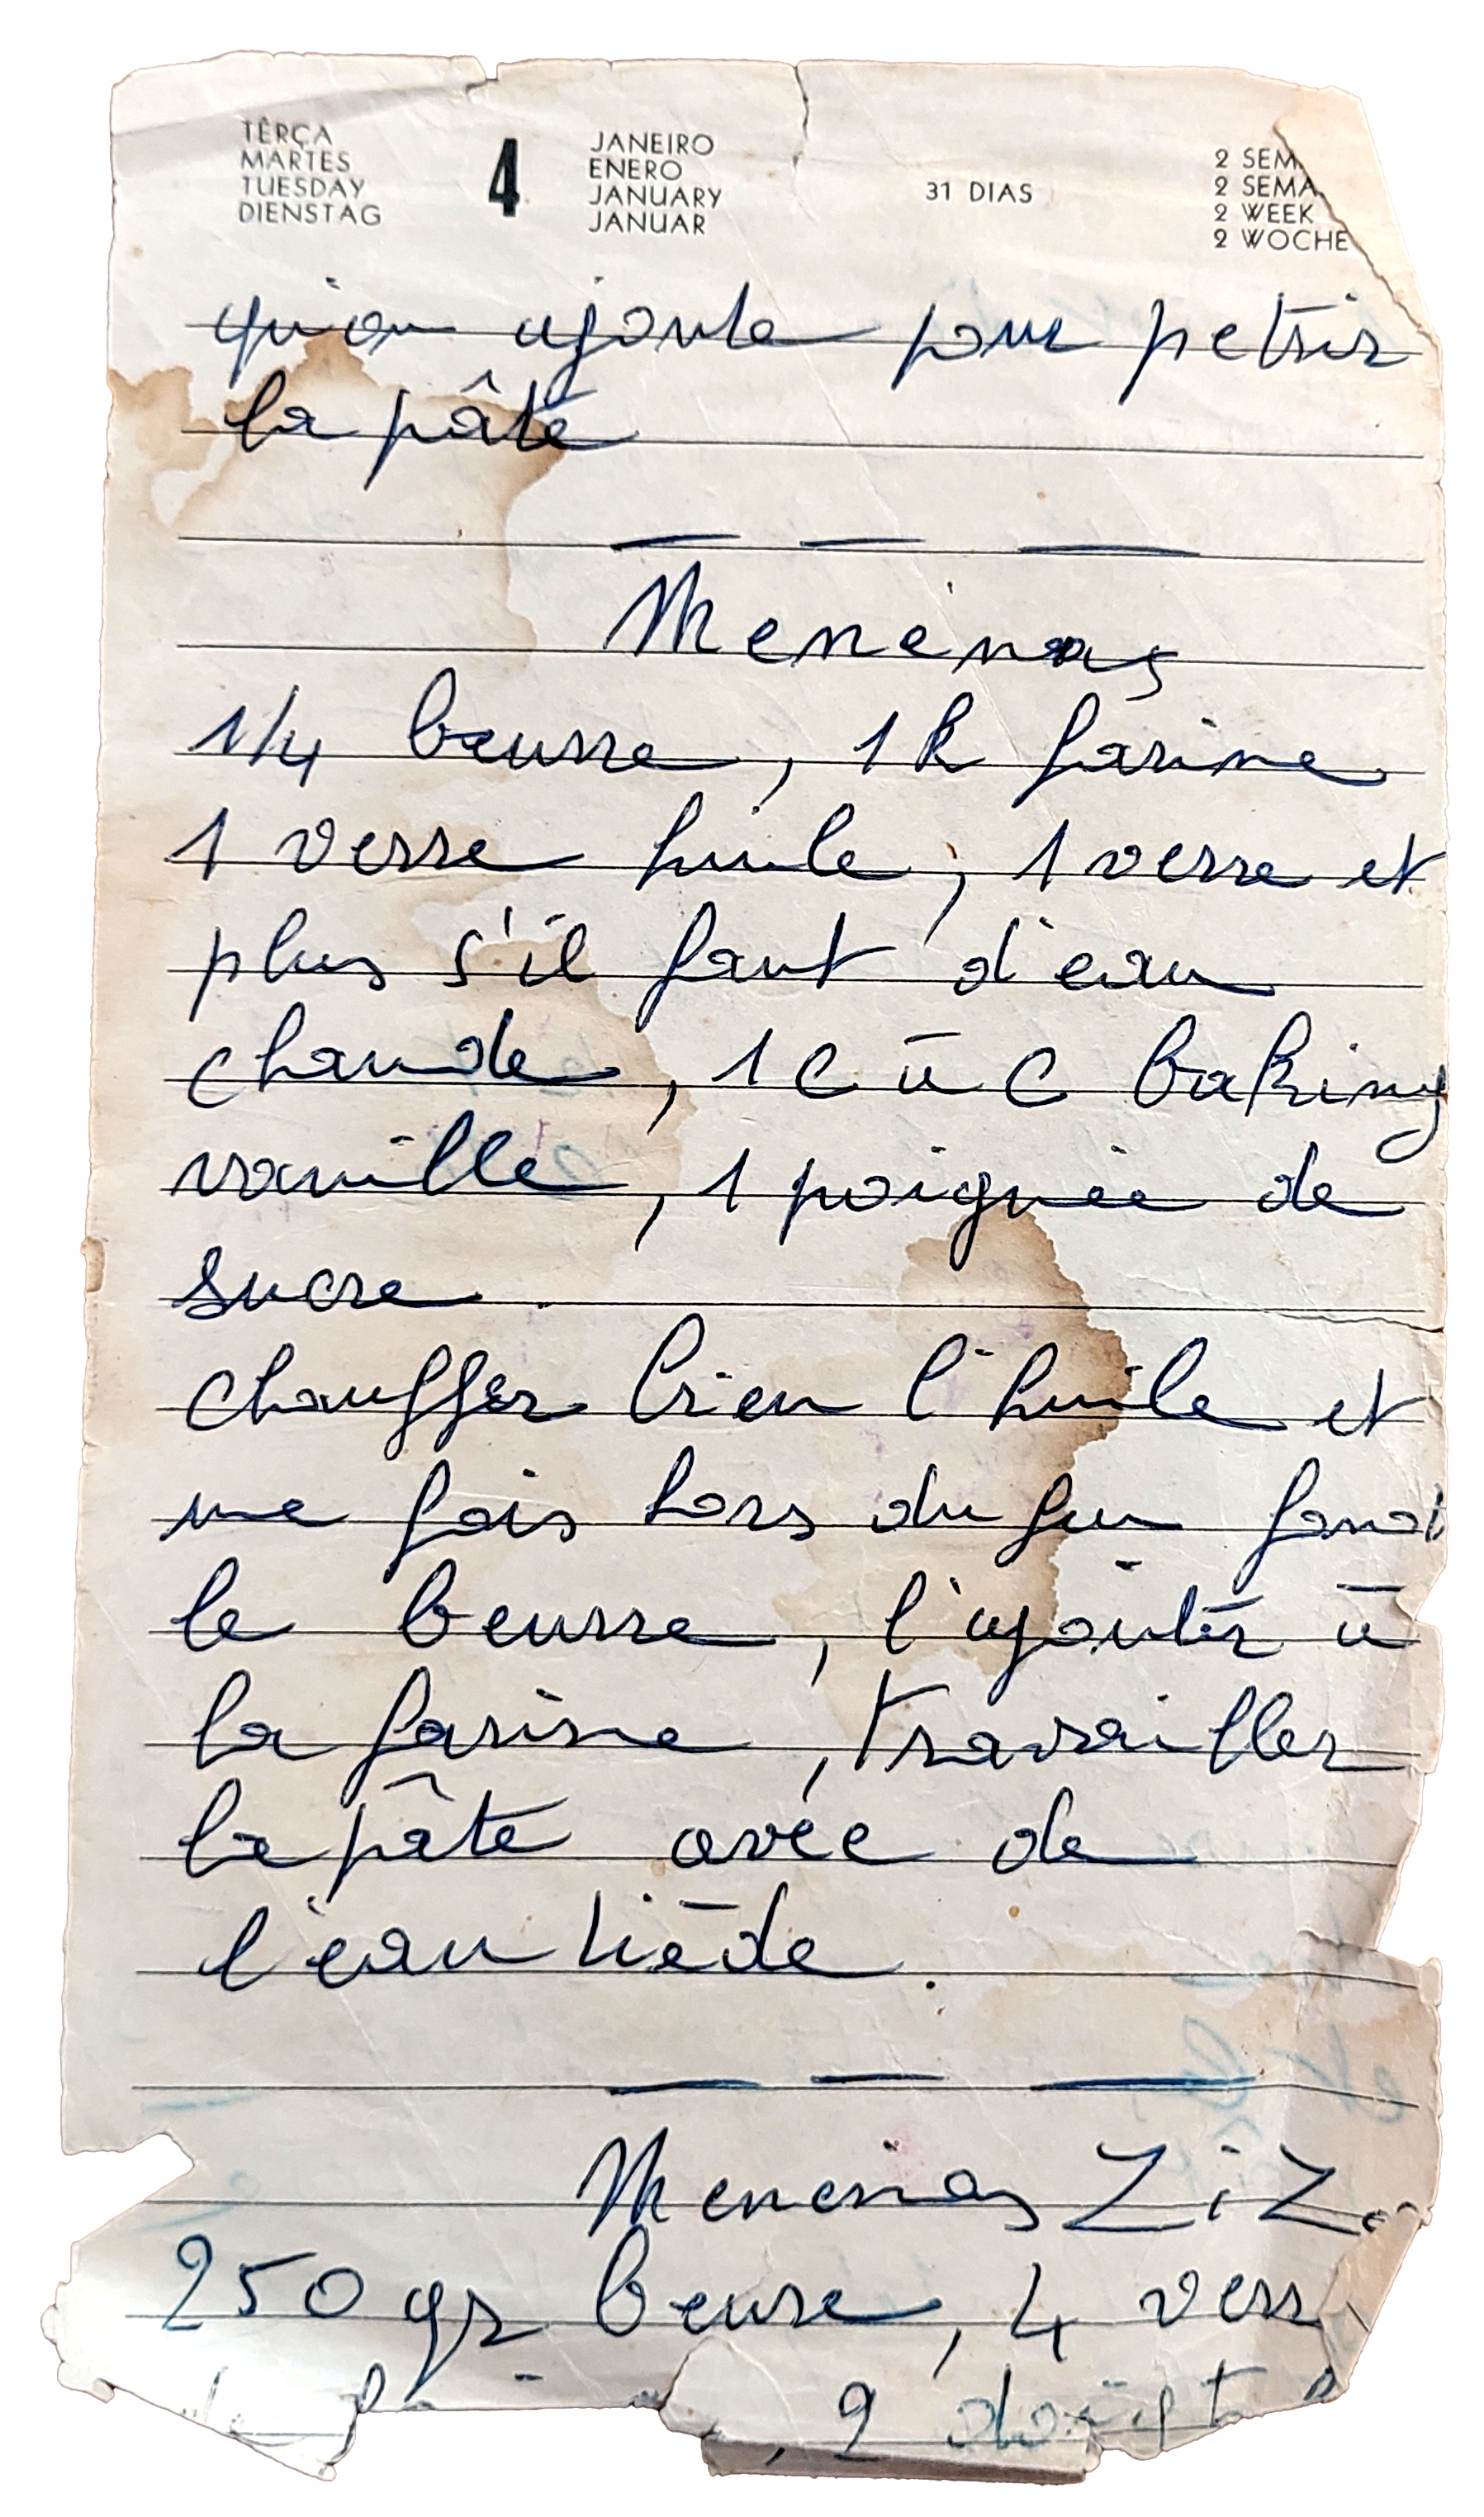
\includegraphics[width=8cm]{./recettes/edités/Menenas.jpg}}; 
\end{tikzpicture}\clearpage\thispagestyle{empty}
% \begin{tikzpicture}[remember picture,overlay]
% \fill[black] (-3,3.5) rectangle (14,-21.5);
% \end{tikzpicture}
\clearpage

\chapter*{Menenas}

\section{Ingrédients originaux}

\begin{itemize}
\item 1/4 beurre
\item 1 kg farine
\item 1 verre huile
\item 1 verre et plus s’il faut d’eau chaude
\item 1 c à c baking
\item vanille
\item 1 poignée de sucre
\end{itemize}

\section{Préparation adaptée}

Chauffez l’huile et, hors du feu, faites fondre le beurre puis versez sur la farine. Mélangez avec le sucre, la vanille et la levure (\textsc{b.,p.}). Ajoutez de l’eau tiède progressivement jusqu’à obtenir une pâte souple et homogène. Préparez la farce en écrasant les dattes (hydratées si nécessaire) en une pâte. Façonnez des portions, garnissez et refermez. Disposez sur une plaque et faites cuire à 180°\,\textsc{c} pendant 20--30 minutes, jusqu’à légère coloration.

\chapter{Menenas}

\section{Ingredientes originais}

\begin{itemize}
\item 1/4 de manteiga
\item 1 kg de farinha
\item 1 copo de óleo
\item 1 copo e mais, se necessário, de água quente
\item 1 colher de chá de fermento químico
\item baunilha
\item 1 punhado de açúcar
\end{itemize}

\section{Modo de preparo adaptado}

Aqueça o óleo e, fora do fogo, derreta a manteiga e despeje sobre a farinha. Misture com o açúcar, a baunilha e o fermento. Acrescente água morna aos poucos até obter uma massa macia e homogênea. Prepare o recheio amassando tâmaras (hidratadas, se necessário) até formar uma pasta. Modele porções, recheie e feche. Disponha em uma assadeira e leve ao forno a 180°\,\textsc{c} por 20--30 minutos, até dourar levemente.

